% Apéndices: elaboración propia. Se numeran A, B, ... (\apendice en tesis-usach.tex)

\chapter{Trazabilidad de los avances}
\label{ap:avances}

Las fichas de cada avance están en la Sección~\ref{sec:iteraciones}. Este apéndice resume qué requisitos aborda cada uno, con el mismo formato de \citet{figueroa2025arquitectura} (Tablas~\ref{tab:matriz_rf} y \ref{tab:matriz_rnf}), y el registro completo de los hallazgos según la fase de reparación de MECIVA PS (Tabla~\ref{tab:hallazgos}).

\newcommand{\avsi}{$\checkmark$}
\begin{table}[H]
\centering
\caption{Requisitos funcionales abordados en cada avance.}
\label{tab:matriz_rf}
\footnotesize
\begin{tabular}{l c c c c c c c}
\toprule
Requisito & P-01 & P-02 & P-03 & P-04 & P-05 & P-06 & P-07 \\ \midrule
N1, N2, N3, RFCO12 & \avsi & & & & & & \avsi \\
N4, N5, N6, N8 & & \avsi & & & & & \avsi \\
N7 & & & \avsi & & & & \avsi \\
FD1 & & & \avsi & & & & \avsi \\
C1, C2, C3, C7, C9, C10 & & \avsi & & & & & \avsi \\
C11 & & \avsi & & & & \avsi & \avsi \\
C5, C6, C8, C12 & & & & & & \avsi & \avsi \\
G1, G2, G3 & & & & \avsi & & & \avsi \\
RO1--RO7 & & & & & \avsi & & \avsi \\
B1--B13 & & & & & & \avsi & \avsi \\
RFS1, RFS2 & & & & & & \avsi & \avsi \\
RFS3, RFS5--RFS8 & & & \avsi & & & & \avsi \\
RFS4 & & & & & \avsi & & \avsi \\
U1, U3 & & & \avsi & & & & \avsi \\
U2 & & & & \avsi & & & \avsi \\ \bottomrule
\end{tabular}
\fuente{Elaboración propia a partir de las fichas de los avances.}
\end{table}

\begin{table}[H]
\centering
\caption{Requisitos no funcionales abordados en cada avance.}
\label{tab:matriz_rnf}
\footnotesize
\begin{tabular}{l c c c c c c c}
\toprule
Requisito & P-01 & P-02 & P-03 & P-04 & P-05 & P-06 & P-07 \\ \midrule
RNF-01 & \avsi & \avsi & \avsi & \avsi & \avsi & \avsi & \avsi \\
RNF-02 & \avsi & \avsi & & & \avsi & & \avsi \\
RNF-03 & & & & & & & \avsi \\
RNF-04 & \avsi & \avsi & & \avsi & & & \avsi \\
RNF-05 & \avsi & \avsi & & & \avsi & & \avsi \\
RNF-06 & & & \avsi & \avsi & & \avsi & \avsi \\
RNF-07 & & & \avsi & & & & \avsi \\
RNF-08 & & & & & & \avsi & \avsi \\ \bottomrule
\end{tabular}
\fuente{Elaboración propia a partir de las fichas de los avances.}
\end{table}

% Ficha extraída de datos/tabla_prototipos.tex (Hallazgos (fase de reparación MECIVA PS))
\begin{table}[H]
\centering
\caption{Hallazgos de la verificación.}
\label{tab:hallazgos}
\begin{tabularx}{\textwidth}{l X l X}
\toprule
ID & Descripción & Estado & Justificación o Solución \\ \midrule
H-01 & Al calibrar con Hand Skin la vista de la cámara aparece rotada 180$^{\circ}$. HandSkinRecognition.cs rotaba siempre la imagen porque la cámara del laboratorio estaba montada invertida; el port conservó esa rotación fija, solo en ese plug-in (Color Pen y Mouse no rotan), así que la vista previa y las coordenadas de calibración quedaban al revés con cualquier otra cámara. & SF & La rotación pasa a ser una opción común de los tres plug-ins (rotate\_180, por defecto desactivada) que se aplica una sola vez al frame; vista previa, coordenadas y recorte comparten orientación. Casilla nueva <<Rotar la imagen 180$^{\circ}$>> en Gestos para el montaje invertido del laboratorio. \\ \midrule
H-02 & ConsistencyPlugin guardaba cada cambio con saveIncr(). Con PyMuPDF 2.1, desde el segundo guardado incremental el PDF queda con la xref dañada; al reabrirlo PyMuPDF lo <<repara>> y se pierden los resaltados, comentarios y marcadores guardados antes. En pantalla no se notaba porque el documento en memoria seguía correcto. & SF & Cada guardado escribe una copia completa en un archivo temporal, reemplaza el original y vuelve a abrirlo (se mantiene el respaldo .bac). Si otro programa tiene el PDF bloqueado (Windows), se reintenta y luego se informa con un mensaje claro. \\ \midrule
H-03 & Al pulsar los botones de carpeta o las casillas de Rastreo ocular aparecía <<'bool' object has no attribute 'mapToGlobal'>>. La ayuda contextual se conectaba con lambda w=widget, t=text a la señal clicked; en los botones, clicked(bool) entrega checked y Qt lo pasaba como primer argumento, reemplazando w por False. La acción del botón sí se ejecutaba, pero cada clic dejaba una excepción. & SF & La ayuda por clic queda solo para los íconos de información; los botones y casillas la muestran al pasar el mouse. La lambda ignora los argumentos de la señal (lambda *\_, w=widget, t=text). Se corrige desde P-05, primer avance con esos controles, hasta P-07. \\ \bottomrule
\end{tabularx}
\fuente{Elaboración propia, 2026.}
\end{table}


\chapter{Mediciones de los prototipos}
\label{ap:mediciones}

La Tabla~\ref{tab:resumen_mediciones} resume el tipo de medición y el resultado principal de cada prototipo. El detalle (protocolo, fórmula, parámetros y todas las métricas) está en avances/P-00\_prototipos\_desechables/evidencias/MEDICIONES.md, generado junto con los valores de este documento.

\begin{table}[H]
\centering
\caption{Resumen de las mediciones de los prototipos.}
\label{tab:resumen_mediciones}
\footnotesize
\begin{tabularx}{\textwidth}{l l >{\raggedright\arraybackslash}X}
\toprule
ID & Tipo & Resultado principal \\ \midrule
F1 & \FUnoTipo & \pendiente{FPS y latencia con las cámaras} \\
F2 & \FDosTipo & Eficacia Otsu \FDosEficaciaPct\%; adaptativo \FDosEficaciaAdaptativoPct\% \\
F3 & \FTresTipo & CER \FTresCerLimpioPct\% / WER \FTresWerLimpioPct\% (sin preproceso: \FTresCerSinPreprocesoPct\% / \FTresWerSinPreprocesoPct\%) \\
F4 & \FCuatroTipo & Éxito \FCuatroExitoPct\%, RMSE \FCuatroRmsePx~px \\
F5 & \FCincoTipo & Detección \FCincoDeteccionPct\% sin rojo proyectado; \FCincoDeteccionRojoPct\% con rojo \\
F6 & \FSeisTipo & IoU \FSeisIouPct\%, punta correcta \FSeisPuntaOkPct\% \\
F7 & \FSieteTipo & Error de reproyección \FSieteErrorPx~$\pm$~\FSieteErrorSdPx~px \\
F9 & \FNueveTipo & \pendiente{latencia de eventos} \\
F10 & \FDiezTipo & Pérdida \FDiezPerdidaPct\%, \textit{jitter} \FDiezJitterMs~ms \\
F11 & \FOnceTipo & \FOnceFallas{} fallas en \FOnceCargas{} cargas, \FOnceTiempoMs~ms \\
F12 & \FDoceTipo & \FDoceVoluntariasPct\% voluntarias, \FDoceAccidentalesPorMin{} accidentales/min \\
F13 & \FTreceTipo & \FTreceTiempoMs~ms por cuadro \\
F14 & \FCatorceTipo & Coherencia \FCatorceCoherenciaPct\% \\
F15 & \FQuinceTipo & \FQuincePersistidas{}/\FQuinceAnotaciones{} persistidos, \FQuinceTiempoMs~ms \\
F16 & \FDieciseisTipo & \FDieciseisDetectadasPct\% detectadas, \FDieciseisErrorPt~pt \\
F17 & \FDiecisieteTipo & Exactitud \FDiecisieteExactitudPct\%, IoU \FDiecisieteIouPct\% \\
F24 & \FVeinticuatroTipo & \pendiente{exactitud de comandos} \\
F25 & \FVeinticincoTipo & \pendiente{palabras por minuto} \\
F27 & \FVeintisieteTipo & \FVeintisieteTiempoMs~ms por cuadro \\ \bottomrule
\end{tabularx}
\fuente{Elaboración propia, mediciones/medir\_prototipos.py (P-00), \MedicionFecha.}
\end{table}

Para repetir las mediciones en el PC y agregar las de hardware:
\begin{verbatim}
cd avances\P-00_prototipos_desechables
python mediciones\medir_prototipos.py --pdf ruta\al\documento.pdf --camara 0
python ..\..\tesis\datos\actualizar_datos.py ..
\end{verbatim}
El segundo comando copia los valores nuevos a datos/, y al recompilar el documento todas las tablas y fichas se actualizan.

\chapter{Comparación de la interfaz}
\label{ap:interfaz}

Las figuras siguientes comparan la interfaz de EDDIE-2023, reproducida a partir de sus archivos .Designer.cs, con la versión en Python.

\begin{figure}[H]
\centering
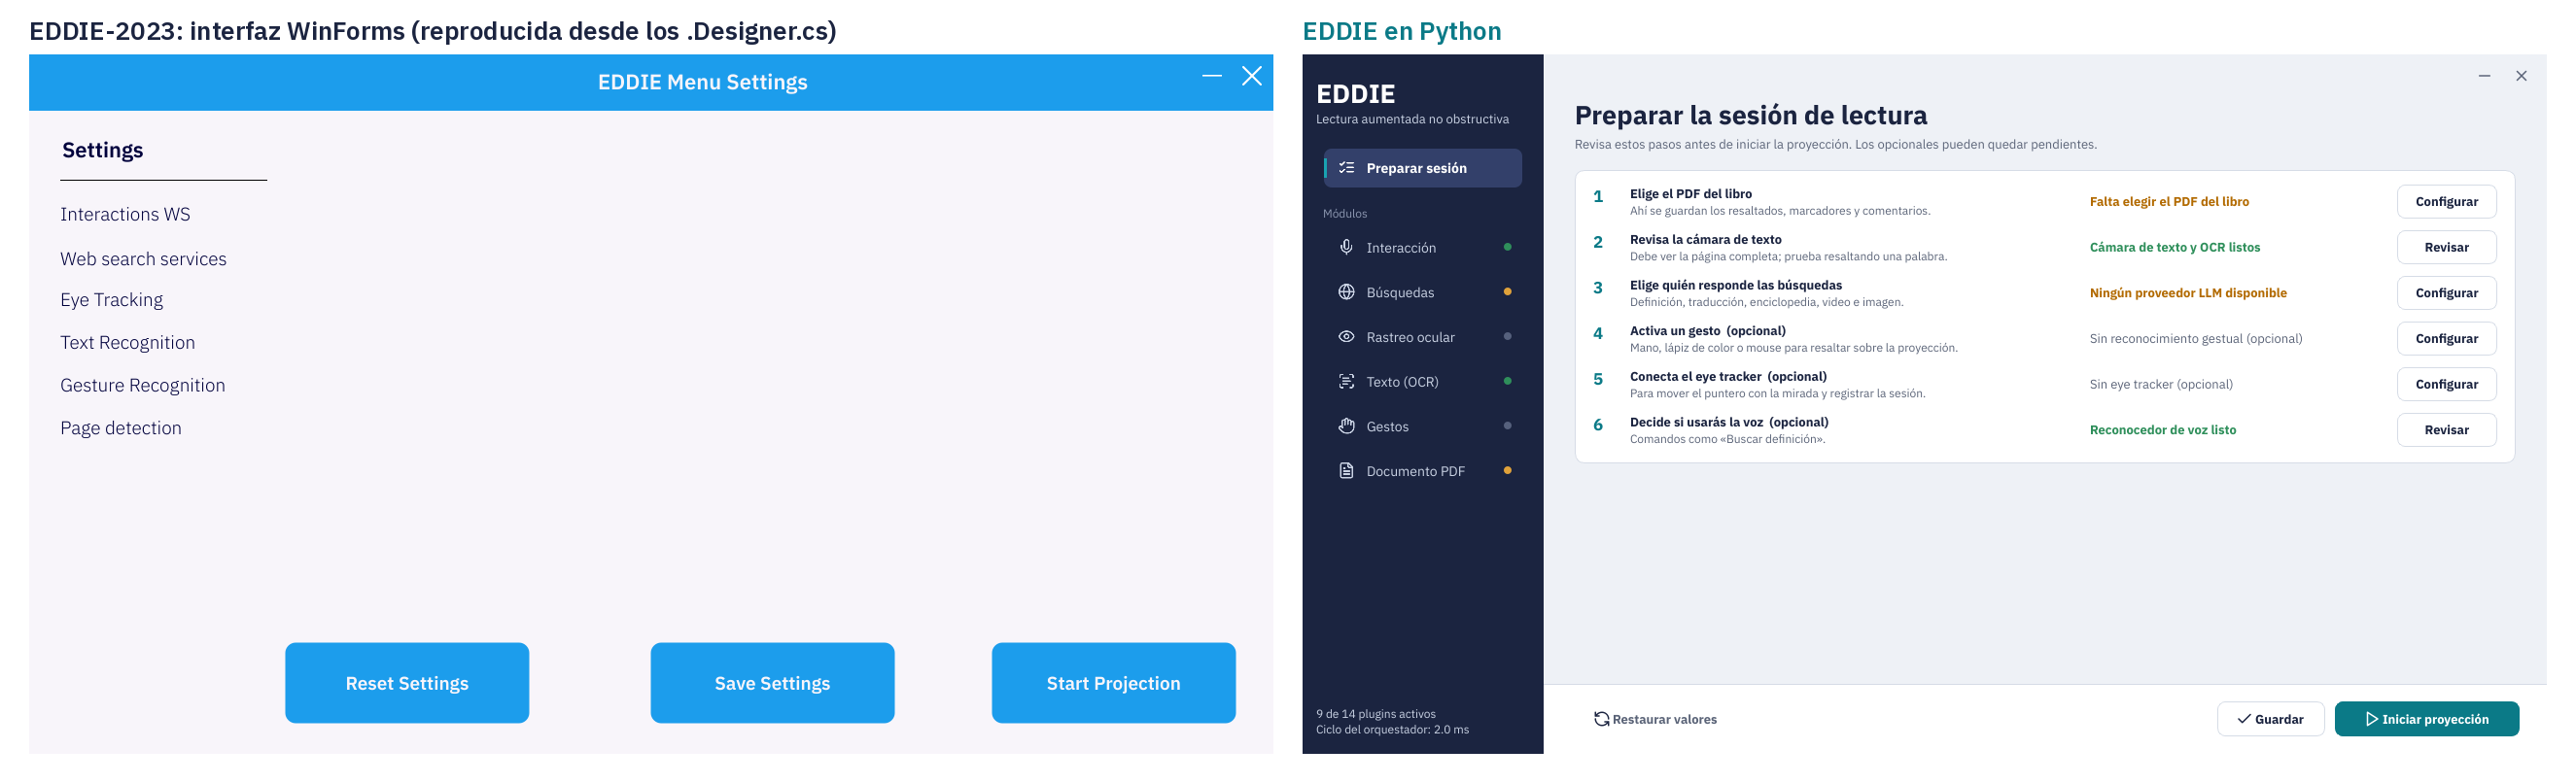
\includegraphics[width=\textwidth]{figuras/comparacion_inicio.png}
\caption{Pantalla de inicio: EDDIE-2023 (izquierda) y versión en Python (derecha).}
\fuente{Elaboración propia.}
\end{figure}

\begin{figure}[H]
\centering
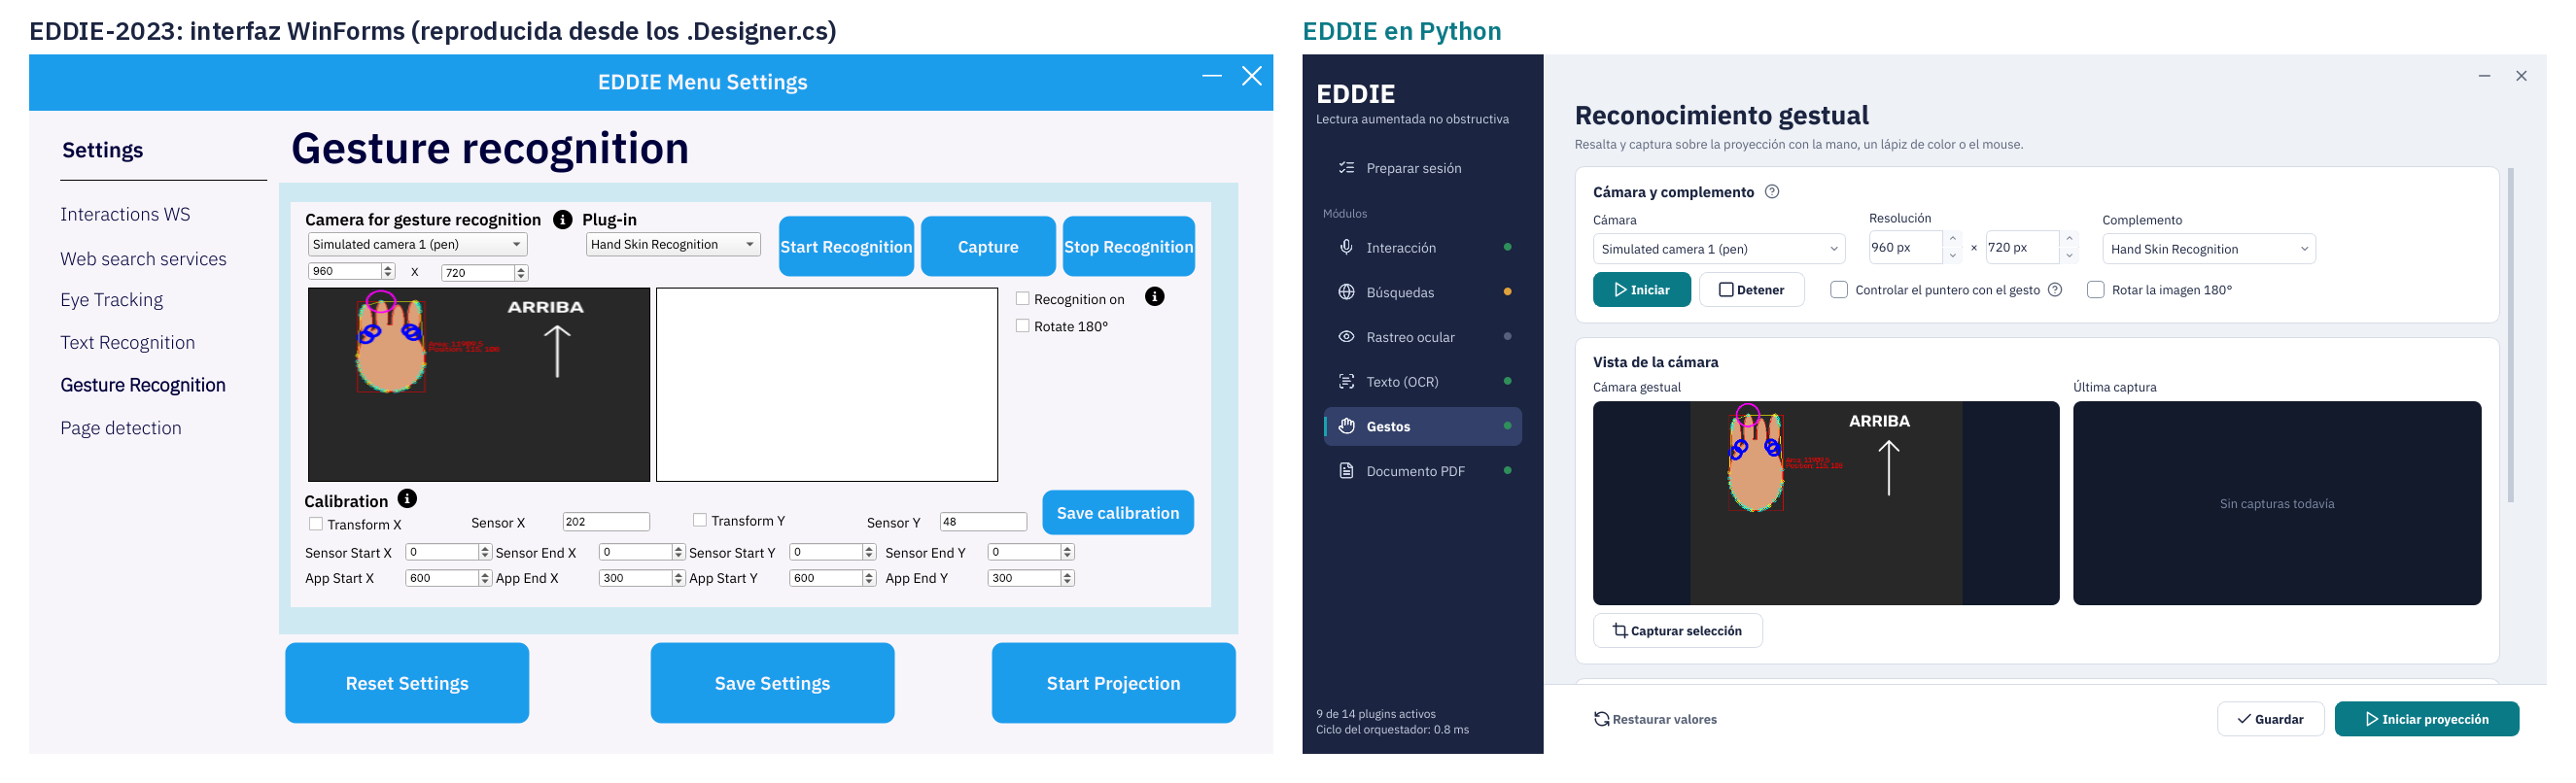
\includegraphics[width=\textwidth]{figuras/comparacion_gestos.png}
\caption{Configuración de gestos: EDDIE-2023 (izquierda) y versión en Python (derecha).}
\fuente{Elaboración propia.}
\end{figure}

\begin{figure}[H]
\centering
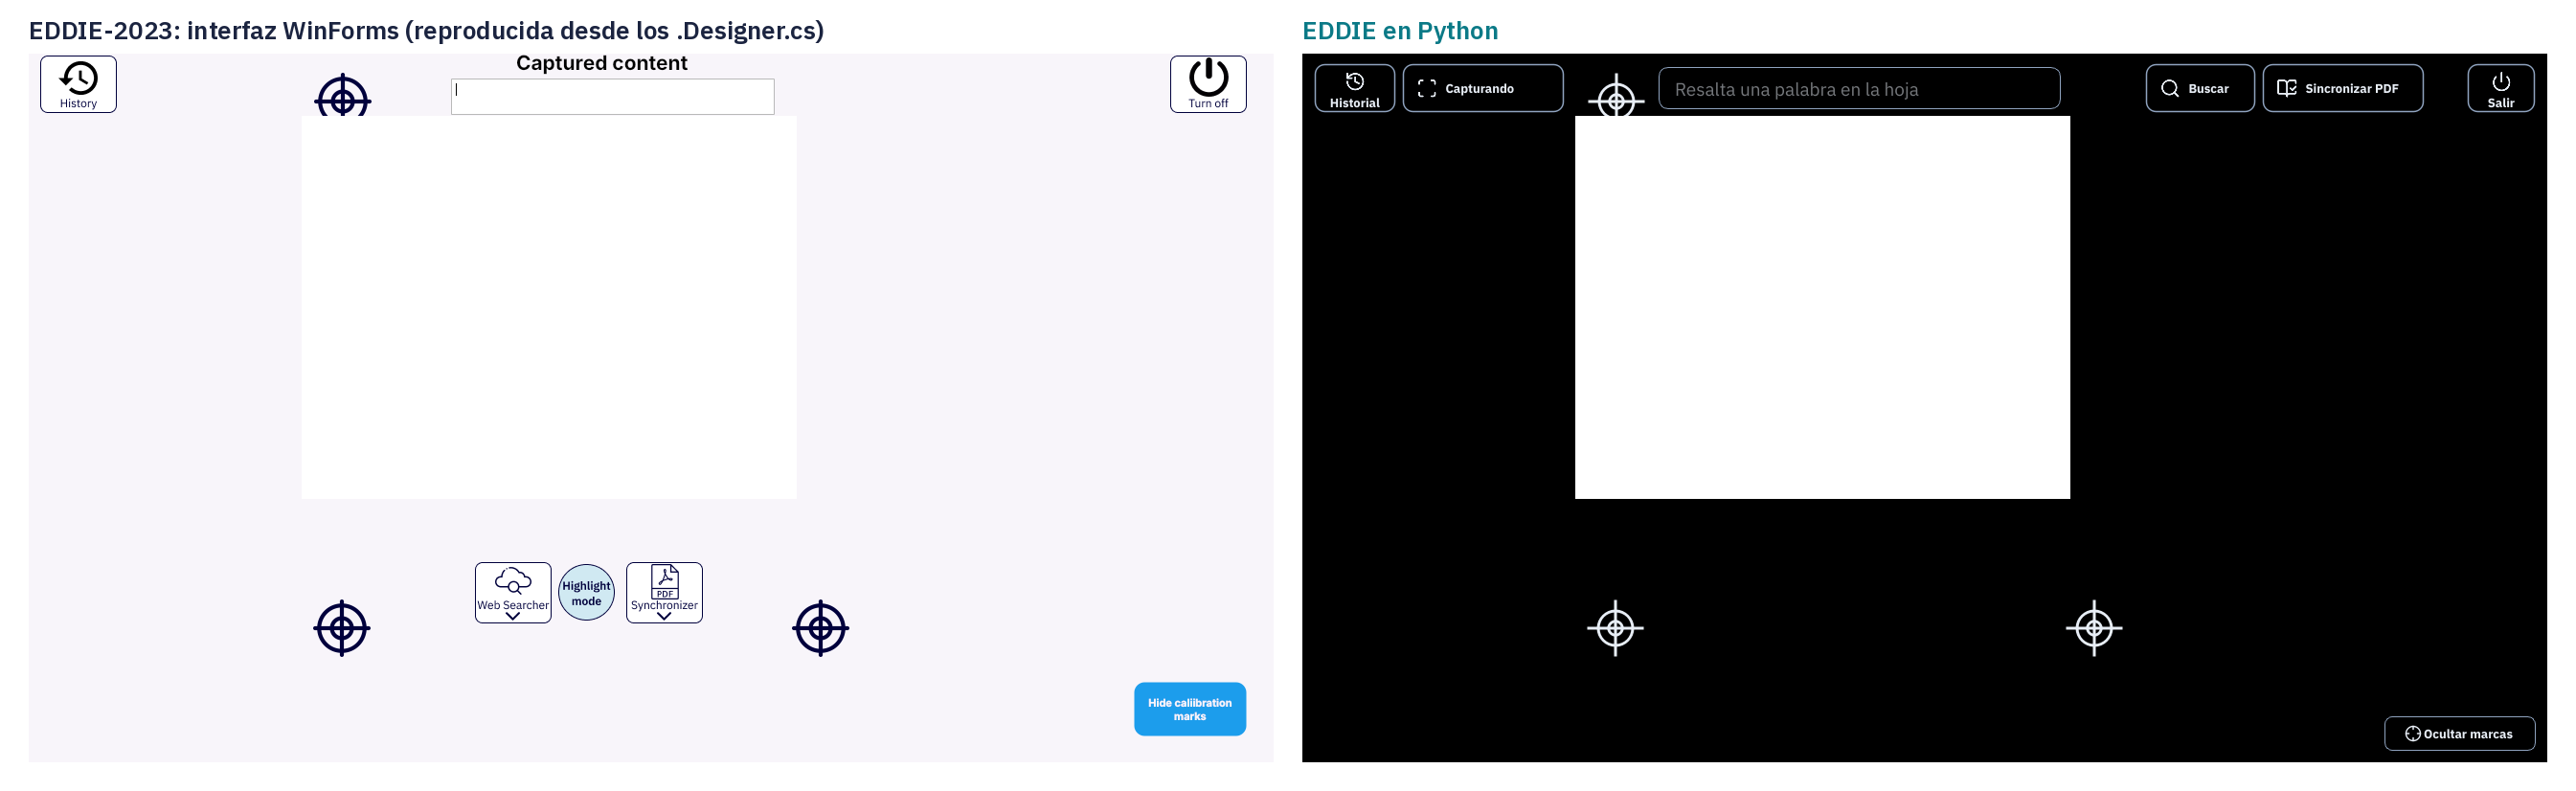
\includegraphics[width=\textwidth]{figuras/comparacion_proyeccion.png}
\caption{Pantalla proyectada: EDDIE-2023 (izquierda) y versión en Python (derecha).}
\fuente{Elaboración propia.}
\end{figure}

\chapter{Manual de instalación y uso}
\label{ap:manual}

\section{Instalación}

\begin{enumerate}
  \item Instalar Python 3.12 (64 bits) y, para el reconocimiento de texto, Tesseract-OCR con el idioma español.
  \item En la carpeta del proyecto:
\begin{verbatim}
python -m venv .venv
.venv\Scripts\activate
pip install -r requirements.txt
\end{verbatim}
  \item Para las búsquedas, copiar \nolinkurl{config/secrets.example.json} como \nolinkurl{config/secrets.json} y pegar la clave de Google AI Studio, o definir la variable GEMINI\_API\_KEY. Este archivo no se sube al repositorio.
  \item Para el rastreo ocular, abrir GazePoint Control o EyeTribe Server antes de conectar el eye tracker desde la aplicación.
\end{enumerate}

\section{Ejecución}

\begin{verbatim}
python main.py              # con el hardware del laboratorio
python main.py --sim        # con cámaras y eye tracker simulados
python -m pytest            # pruebas automatizadas
python tools\generar_evidencias.py   # evidencias
\end{verbatim}

\section{Uso}

\begin{enumerate}
  \item Al abrir, la pantalla de inicio muestra los pasos para preparar la sesión y el estado de cada módulo; cada paso lleva a su página.
  \item En \textit{Texto} y \textit{Gestos}, elegir la cámara y la resolución. En gestos, elegir el complemento (lápiz, mano o mouse), iniciarlo y calibrar apuntando a la cruz superior izquierda y luego a la inferior derecha.
  \item En \textit{Documento PDF}, elegir el PDF del libro.
  \item En \textit{Rastreo ocular}, elegir el eye tracker, la retícula y el registro CSV, y pulsar \textit{Aplicar y conectar}.
  \item Guardar e iniciar la proyección. En la proyección, resaltar una palabra; el texto reconocido aparece en el campo superior y los botones de búsqueda entregan definición, traducción, enciclopedia, video o imagen. \textit{Sincronizar PDF} abre las herramientas de consistencia papel--PDF.
\end{enumerate}

Los ajustes se guardan en config/user\_settings.json, las búsquedas en CSV\_registro\_actividades/ y cada acción del orquestador con su latencia en logs/.
